\section{Transformations}

\begin{definition}[\textit{Projective mapping}]
    A projective mapping between a projective plane $\mathbb{P}^2$ and another projective plane $\mathbb{P}^{\prime 2}$ is an invertible mapping which preserves co-linearity:
    \[h:\mathbb{P}^2 \rightarrow \mathbb{P}^{\prime 2}, x^\prime=h(\mathbf{x}),\mathbf{x}_1,\mathbf{x}_2,\mathbf{x}_3 \textnormal{ are colinear}\]
    \[\Leftrightarrow\]
    \[\mathbf{x}_1^\prime=h(\mathbf{x}_1),\mathbf{x}_2^\prime=h(\mathbf{x}_2),\mathbf{x}_3^\prime=h(\mathbf{x}_3) \textnormal{ are colinear}\]
\end{definition}
Projective mapping is also called projectivity or homography. 
\begin{theorem}
    A mapping $h:\mathbb{P}^{2} \rightarrow \mathbb{P}^{\prime 2}$ is projective if and only if there exists an invertible $3 \times 3$ matrix $\mathbf{H}$ such that for any point in $\mathbb{P}^{2}$ represented by the vector $\mathbf{x}$, is $h(\mathbf{x})=\mathbf{Hx}$, where: 
    \[\mathbf{H}=\begin{bmatrix}
        h_{11} & h_{12} & h{13} \\
        h_{21} & h_{22} & h{23} \\
        h_{31} & h_{32} & h{33} 
    \end{bmatrix}\]
\end{theorem}
Projective mappings are linear when expressed in homogeneous coordinates, but they do not exhibit linearity when represented in Cartesian coordinates.

According to the theorem, if we have $h(\mathbf{x})=\mathbf{x}^\prime=\mathbf{Hx}$, then multiplying the matrix $\mathbf{H}$ by any nonzero scalar $\lambda$ still satisfies the relation for the same points, giving us $\mathbf{x}^\prime=\lambda \mathbf{Hx}$. 
Therefore, any nonzero scalar multiple of the matrix $\mathbf{H}$ represents the same projective mapping as $\mathbf{H}$.
As a result, we can conclude that $\mathbf{H}$ is a homogeneous matrix.
Despite having nine entries, it possesses only eight degrees of freedom, specifically the ratios between its elements. 
Consequently, we can estimate $\mathbf{H}$ using just four point correspondences.
Each point correspondence, expressed as $\mathbf{x}^\prime=\mathbf{Hx}$, provides two independent equations in this estimation process.
\begin{definition}[\textit{Homography}]
    A homography transforms various geometric entities as follows:
\end{definition}
\begin{enumerate}
    \item It maps a point $\mathbf{x}$ to a point $\mathbf{x}^\prime$, where the transformation is expressed as: 
        \[\mathbf{x} \rightarrow \mathbf{Hx}=\mathbf{x}^\prime\]
    \item It maps a line $\mathbf{l}$ to a line $\mathbf{l}^\prime$, and this transformation is represented as: 
        \[\mathbf{l} \rightarrow \mathbf{H}^{-T} \mathbf{l}=\mathbf{l}^\prime\]
    \item It maps a conic $\mathbf{C}$ to a conic $\mathbf{C}^\prime$, and the transformation is given by: 
        \[\mathbf{C} \rightarrow \mathbf{H}^{-T} \mathbf{CH}^{-1}=\mathbf{C}^\prime\]
    \item It maps a dual conic $\mathbf{C}^\ast$ to a dual conic $C^{\ast\prime}$, with the transformation being: 
        \[\mathbf{C}^\ast \rightarrow \mathbf{HC}^\ast \mathbf{H}^{T}=\mathbf{C}^{\ast\prime}\]
\end{enumerate}
\begin{proof}[Proof of mapping two]
    To transform the equation of the line in terms of $\mathbf{x}$, given by $\mathbf{l}^T\mathbf{x}=0$, into a constraint on $\mathbf{x}^\prime=\mathbf{Hx}$, we combine the two equations, resulting in a linear equation on $\mathbf{x}^\prime$: 
    \[\mathbf{l}^{\prime T}\mathbf{x}^\prime=0\]
    Here, $\mathbf{l}^{\prime T}=\mathbf{l}^{T}\mathbf{H}^{-1}$. 
    Thus, we have:
    \[\mathbf{l}^\prime=\mathbf{H}^{-T}\mathbf{l}\]
\end{proof}
\begin{proof}[Proof of mapping three]
    To transform the equation of the conic in terms of $\mathbf{x}$, given by $\mathbf{x}^{T}\mathbf{Cx}=0$, into a constraint on $\mathbf{x}^\prime=\mathbf{Hx}$, we have $\mathbf{x}=\mathbf{H}^{-1}\mathbf{x}^\prime$ and $\mathbf{x}^{T}=\mathbf{x}^{\prime T}\mathbf{H}^{-T}$. 
    Combining these three equations, we obtain a linear equation on $\mathbf{x}^\prime$: 
    \[\mathbf{x}^{\prime T}\mathbf{C}^\prime \mathbf{x}^\prime=0\]
    Hence, we have:
    \[\mathbf{C}^\prime=\mathbf{H}^{-T} \mathbf{CH}^{-1}\]
\end{proof}
\begin{proof}[Proof of mapping four]
    For the transformation of a dual conic, we apply the same idea, yielding:
    \[\mathbf{C}^{\ast\prime}=\mathbf{HC}^\ast \mathbf{H}^{T}\]
\end{proof}
The point-line incidence is preserved. 
\begin{proof}
    Let $\mathbf{x}$ be a point on the line $\mathbf{l}$. 
    This is expressed as $\mathbf{l}^T\mathbf{x}=0$. 
    When we apply the projective transformation $\mathbf{H}$ to both $\mathbf{x}$ and $\mathbf{l}$, resulting in $\mathbf{Hx}=\mathbf{x}^\prime$ and $\mathbf{H}^{-1}\mathbf{l}=\mathbf{l}^\prime$, they remain incident if $\mathbf{l}^{\prime T}\mathbf{x}^\prime=0$:
    \[\mathbf{l}^{\prime T}\mathbf{x}^\prime=\mathbf{l}^{T}\mathbf{H}^{-1}\mathbf{x}^\prime=\mathbf{l}^{T}\mathbf{H}^{-1}\mathbf{Hx}=\mathbf{l}^{T}x=0\]
\end{proof}

\subsection{Vanishing points and vanishing line}
The point that is common to both parallel lines $\mathbf{l}_1={\begin{bmatrix} a & b & c_1 \end{bmatrix}}^{T}$ and $\mathbf{l}_2={\begin{bmatrix} a & b & c_2 \end{bmatrix}}^{T}$ is the point $\mathbf{x}={\begin{bmatrix} b & -a & 0 \end{bmatrix}}^{T}$. 
This point is situated at infinity along the direction of both lines.
When seeking the common point of the infinite lines $\mathbf{l}_i$, we find that they all share the same point:
\[\mathbf{x}_{\infty}={\begin{bmatrix} b & -a & 0 \end{bmatrix}}^{T}\]
Hence, it becomes apparent that all these lines converge at ${\begin{bmatrix} b & -a & 0 \end{bmatrix}}^{T}$. 

If we apply a projective transformation to all the aforementioned parallel lines $\mathbf{l}_i$, we obtain the transformed lines $\mathbf{l}_i^\prime$. 
The common point $\mathbf{x}_{\infty}$, shared by all lines $\mathbf{l}_i$, is mapped to a point $\mathbf{x}_{\infty}^\prime$ which belongs to each of the lines $\mathbf{l}_i^\prime$. 
\begin{figure}[H]
    \centering
    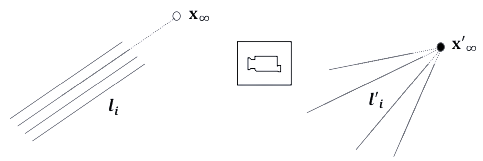
\includegraphics[width=0.5\linewidth]{images/vanishing.png}
\end{figure}
Therefore, we can assert that all lines $\mathbf{l}_i^\prime$ intersect at the point $\mathbf{x}_{\infty}^\prime=\mathbf{Hx}_{\infty}$, referred to as the vanishing point associated with the direction $(b,-a)$ of the parallel lines. 
\begin{theorem}
    The image of a set of parallel lines $\mathbf{l}_i$ is a set of lines $\mathbf{l}_i^\prime$ concurrent at a common point $\mathbf{x}^\prime$ known as the vanishing point of the direction of lines $\mathbf{l}_i$. 
\end{theorem}

By applying a projective transformation to the line at infinity $\mathbf{l}_{\infty}$, we obtain a line $\mathbf{l}_{\infty}^\prime$. 
This line intersects the image all the points at the infinity $\mathbf{x}_{\infty}$ from  the original plane. 
Consequently, the vanishing line $\mathbf{l}_{\infty}^\prime$ can be determined from two vanishing points. 
\begin{figure}[H]
    \centering
    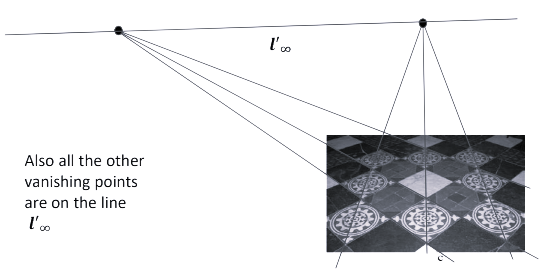
\includegraphics[width=0.5\linewidth]{images/vanishingline.png}
\end{figure}

\subsection{Polarity}
Polarity remains unaltered in the presence of projective mappings.
The polar line $\mathbf{l}=\mathbf{Cx}$ corresponding to a point $\mathbf{x}$ with respect to a conic $\mathbf{C}$ gets mapped to the polar line of the transformed point $\mathbf{x}^\prime = \mathbf{Hx}$ with respect to the transformed conic:
\[\mathbf{C}^\prime=\mathbf{H}^{-T}\mathbf{CH}^{-1}\]
\begin{proof}
    This property holds because:
    \[\mathbf{C}^\prime \mathbf{x}^\prime=\mathbf{H}^{-T}\mathbf{CH}^{-1}\mathbf{Hx}=\mathbf{H}^{-T}\mathbf{Cx}=\mathbf{H}^{-T}\mathbf{l}=\mathbf{l}^\prime\]
    Therefore, the polar line of the transformed point aligns with the polar line of the original point.
\end{proof}
\begin{figure}[H]
    \centering
    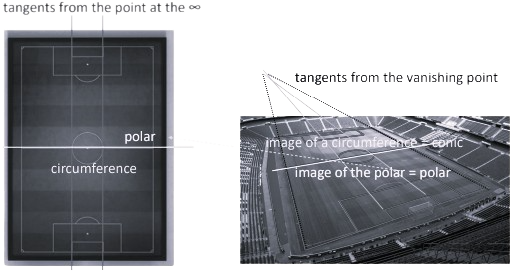
\includegraphics[width=0.75\linewidth]{images/polarity.png}
\end{figure}
In conclusion, as polarity remains intact under projective mappings, conjugacy is similarly preserved, and the relationship $\text{CR}=-1$ is also upheld.

\subsection{Cross ratio}
Given a line defined by four points with the following relationships:
\[\mathbf{x}_1=\propto_1\mathbf{y}+\beta_1\mathbf{z}\]
\[\mathbf{x}_2=\propto_2\mathbf{y}+\beta_2\mathbf{z}\]
The cross ratio is expressed as:
\[\text{CR}_{\mathbf{x}_1,\mathbf{x}_2,\mathbf{y},\mathbf{z}}=\dfrac{\frac{\beta_1}{\alpha_1}}{\frac{\beta_2}{\alpha_2}}\]
Upon applying a projective transformation $\mathbf{H}$ to these four points:
\[\begin{cases}
    \mathbf{y}^\prime=\mathbf{Hy} \\
    \mathbf{z}^\prime=\mathbf{Hz} \\ 
    \mathbf{x}^\prime_1=\mathbf{H}\mathbf{x}_1\propto_1\mathbf{y}^\prime+\beta_1\mathbf{z}^\prime \\
    \mathbf{x}^\prime_2=\mathbf{H}\mathbf{x}_2\propto_2\mathbf{y}^\prime+\beta_2\mathbf{z}^\prime
\end{cases}\]
The coefficients of the linear combination remain the same. 
Hence, the cross ratio is conserved, maintaining its original value:
\[\text{CR}_{\mathbf{x}_1^\prime,\mathbf{x}_2^\prime,\mathbf{y}^\prime,\mathbf{z}^\prime}=\dfrac{\frac{\beta_1}{\alpha_1}}{\frac{\beta_2}{\alpha_2}}=\text{CR}_{\mathbf{x}_1,\mathbf{x}_2,\mathbf{y},\mathbf{z}}\]

\subsection{Isometries}
Isometries possess three degrees of freedom, which include translation denoted as $t$ and the rotation angle represented by $\vartheta$. 
Consequently, the invariants of this transformation encompass lengths, distances, and areas.
\begin{figure}[H]
    \centering
    
\includegraphics[width=0.25\linewidth]{images/isometry.png}
\end{figure}
\begin{definition}
    The \emph{orthogonal matrix} $\mathbf{R}_{\perp}$ is defined as follows: 
    \[\mathbf{R}_{\perp}^{-1}=\mathbf{R}_{\perp}^{T}\]
\end{definition}
Hence, the matrix $\mathbf{H}_I$ for isometries takes the following form:
\[\mathbf{H}_I=
\begin{bmatrix}
    \cos \vartheta & -\sin \vartheta & t_x \\
    \sin \vartheta & \cos \vartheta & t_y \\
    0 & 0 & 1
\end{bmatrix}\]
Here, $
\begin{bmatrix}
    \cos \vartheta & -\sin \vartheta \\
    \sin \vartheta & \cos \vartheta
\end{bmatrix}
=\mathbf{R}_{\perp}$
\begin{figure}[H]
    \centering
    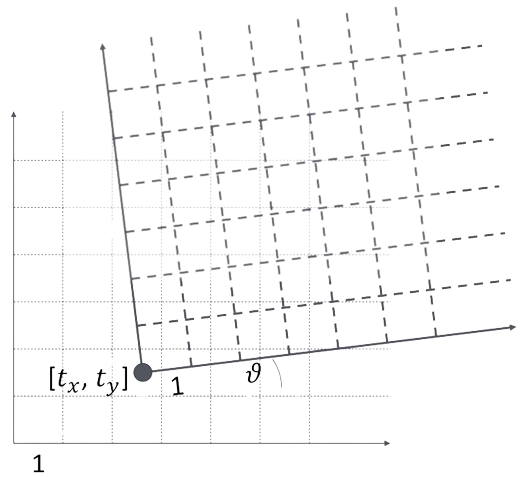
\includegraphics[width=0.25\linewidth]{images/isometry1.png}
    \caption{Isometry}
\end{figure}

\subsection{Similarities}
Similarities are characterized by four degrees of freedom, encompassing the translation, denoted as $t$; the scale, represented by $s$; and the rotation angle, expressed as $\vartheta$.
Consequently, the invariants of this transformation encompass the ratio of lengths and angles.
Furthermore, the circular points $\mathbf{I}$ and $\mathbf{J}$ remain invariant throughout this transformation.
\begin{figure}[H]
    \centering
    
\includegraphics[width=0.2\linewidth]{images/similarity.png}
\end{figure}
Hence, the matrix $\mathbf{H}_S$ for similarities is as follows:
\[\mathbf{H}_I=
\begin{bmatrix}
    s\cos \vartheta & -s\sin \vartheta & t_x \\
    s\sin \vartheta & s\cos \vartheta & t_y \\
    0 & 0 & 1
\end{bmatrix}\]
Here, $
\begin{bmatrix}
    s\cos \vartheta & -s\sin \vartheta \\
    s\sin \vartheta & s\cos \vartheta
\end{bmatrix}
=s\mathbf{R}_{\perp}$
\begin{figure}[H]
    \centering
    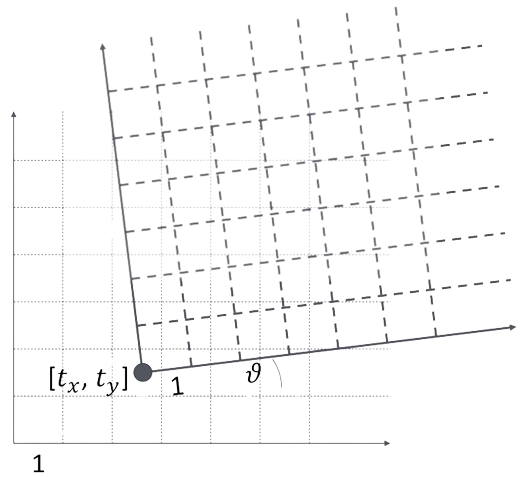
\includegraphics[width=0.25\linewidth]{images/isometry1.png}
    \caption{Similarity}
\end{figure}

\subsection{Affinities}
Affinities exhibit six degrees of freedom, consisting of the sub-matrix $\mathbf{A}$ and the translation component. 
As a result, the invariants of this transformation encompass parallelism, the ratio of parallel lengths, and the ratio of areas. 
The matrix $\mathbf{A}$ is defined as a $2 \times 2$ matrix with a rank of two. 
Additionally, the line at infinity, denoted as $\mathbf{l}_{\infty}$, remains invariant throughout the transformation.
\begin{figure}[H]
    \centering
    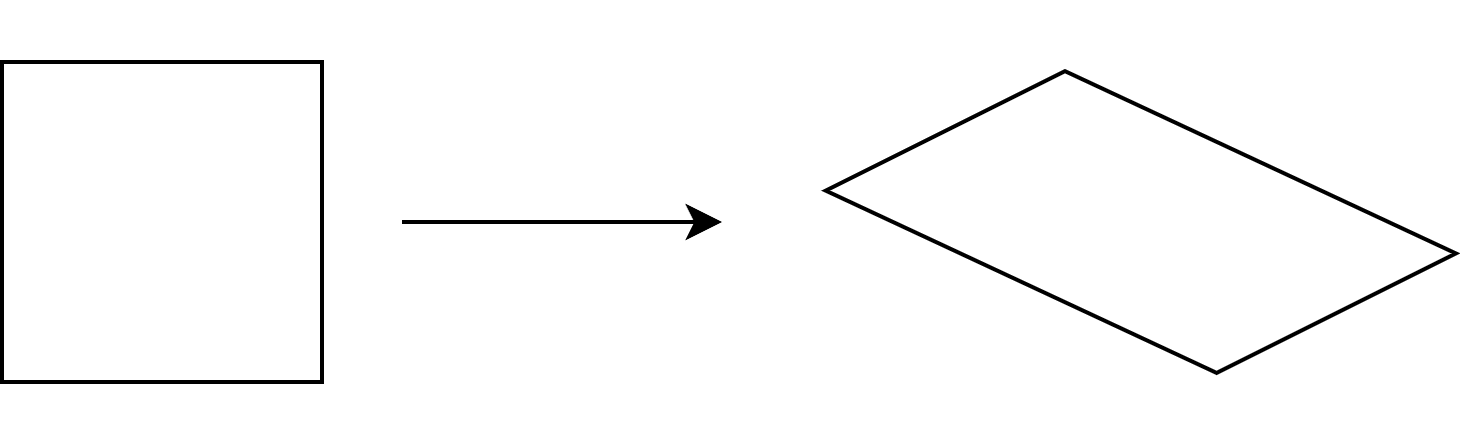
\includegraphics[width=0.25\linewidth]{images/affinities.png}
\end{figure}
Hence, the matrix $\mathbf{H}_A$ for affinities takes the following form:
\[\mathbf{H}_I=
\begin{bmatrix}
    a_{11} & a_{21} & t_x \\
    a_{12} & a_{21} & t_y \\
    0 & 0 & 1
\end{bmatrix}\]
Here, $
\begin{bmatrix}
    a_{11} & a_{21} \\
    a_{12} & a_{21} \\
\end{bmatrix}
=\mathbf{A}$
\begin{figure}[H]
    \centering
    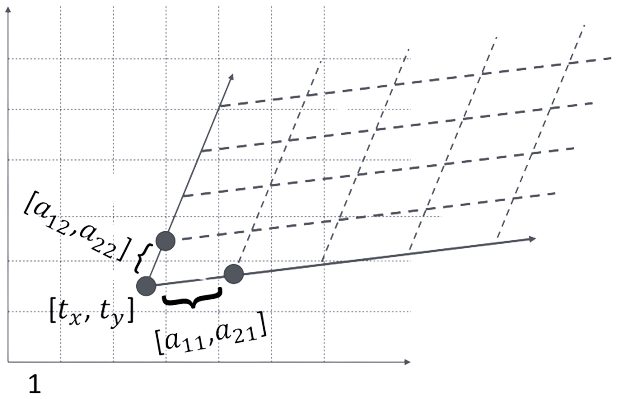
\includegraphics[width=0.3\linewidth]{images/affinities1.png}
\end{figure}


\subsection{Projectivities}
Projectivities possess eight degrees of freedom, encompassing the sub-matrix $\mathbf{A}$, the vector $\mathbf{v}$, and the translation component. 
Therefore, the invariants of this transformation include co-linearity, incidence, and the order of contact.
The matrix $\mathbf{A}$ is defined as a $2 \times 2$ matrix with a rank of two. 
Furthermore, the cross ratio remains invariant throughout this transformation.
\begin{figure}[H]
    \centering
    
\includegraphics[width=0.25\linewidth]{images/projectivities.png}
\end{figure}
Hence, the matrix $\mathbf{H}_P$ for projectivities takes the following form:
\[\mathbf{H}_I=
\begin{bmatrix}
    a_{11} & a_{21} & t_x \\
    a_{12} & a_{21} & t_y \\
    v_1 & v_2 & 1
\end{bmatrix}\]
Here, $
\begin{bmatrix}
    a_{11} & a_{21} \\
    a_{12} & a_{21} \\
\end{bmatrix}
=\mathbf{A}$
\begin{figure}[H]
    \centering
    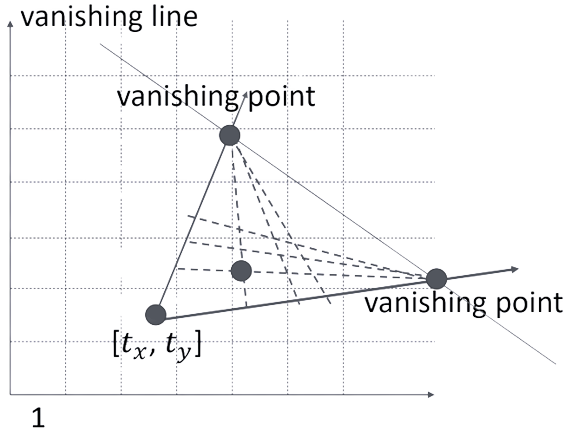
\includegraphics[width=0.25\linewidth]{images/projectivities1.png}
    \caption{Affinity}
\end{figure}